\section{Random Deployment}
\label{sec:random_deployment}

Advanced reactor concepts, like the ones outlined in this work, are often
designed for use cases ranging from industrial steam production to microgrid
integration. Our deployment of these reactors is
a complex problem that requires a nuanced understanding of the energy market,
the regulatory environment, the intended use of the technology, and the
technical capabilities of the reactor.

This random deployment is a proxy for the complexity of the real-world
deployment problem but does not include the nuance of how individual
deployments meet an end user's needs, which will drive the strategic decisions
that utilities and ratepayers behind the meter make in their reactor choices
The random deployment scheme has the potential to capture some of the
complexities in overall market development, but the extent we capture these
details is not explored in this work.

The random deployment scheme is implemented by randomly selecting reactors from
the list of deployable reactors until the demand is covered. We illustrate this
scheme in Figure \ref{fig:random_diagram}, which shows the single loop in the
logic from the top down. There is an irreducible demand that cannot be met
because the power capacity is assumed to be constant. As such the random
deployment scheme, at its best, will meet the demand, but has the potential to
fall short of the demand by one of the smallest capacity reactors. To reduce
the computational cost of this scheme, we have implemented a rough random case
that deploys until the randomly selected reactor exceeds the demand. This rough
approximation is what we couple with the greedy deployment scheme in the
initially random, greedy deployment scheme in Section
\ref{sec:initially_random_greedy}.

\begin{figure}[H]
    \centering
    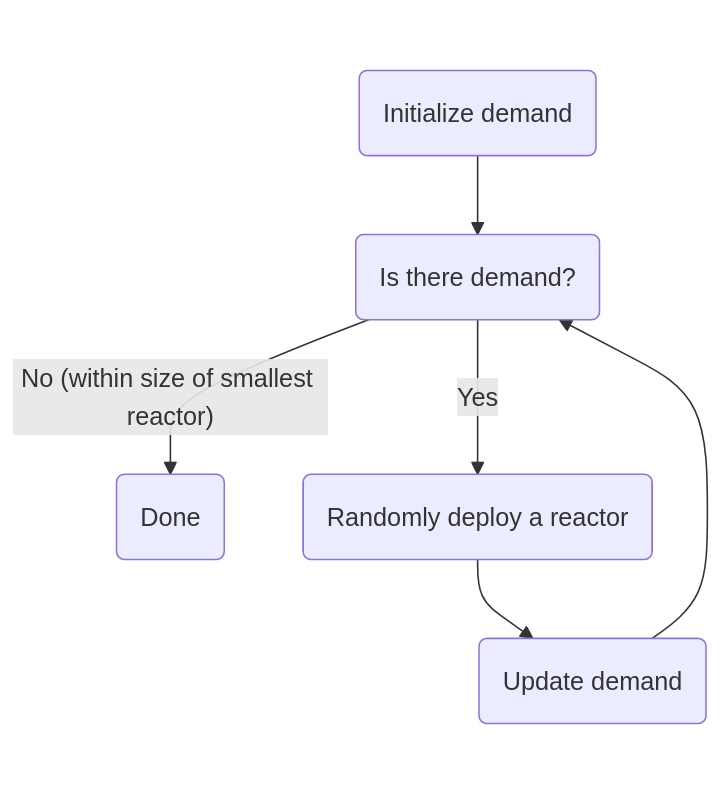
\includegraphics[scale=0.4]{images/schemes/random_diagram.png}
    \caption{Random Deployment Diagram}
    \label{fig:random_diagram}
\end{figure}

The seed, which was set to 20240527121205 for every run for this scheme, for
the random number generator is set by the date and time of the simulation,
which allows for the reproducibility of the results. This scheme is a proxy for
aggregate decisions by actors and would fail to reliably capture individual
actor decisions. This scheme is most useful for scenarios or timescales where
there is a high degree of uncertainty in the deployment of reactors.


\subsection{Number of Reactors}
\label{sec:random_reactors}

% describe the difference between BAU and D2 in terms of metric

% Show total number of reactors multi fuel
\begin{figure}[H]
    \subfloat[No Growth \label{fig:random_mf_ng_reactors}]{%
      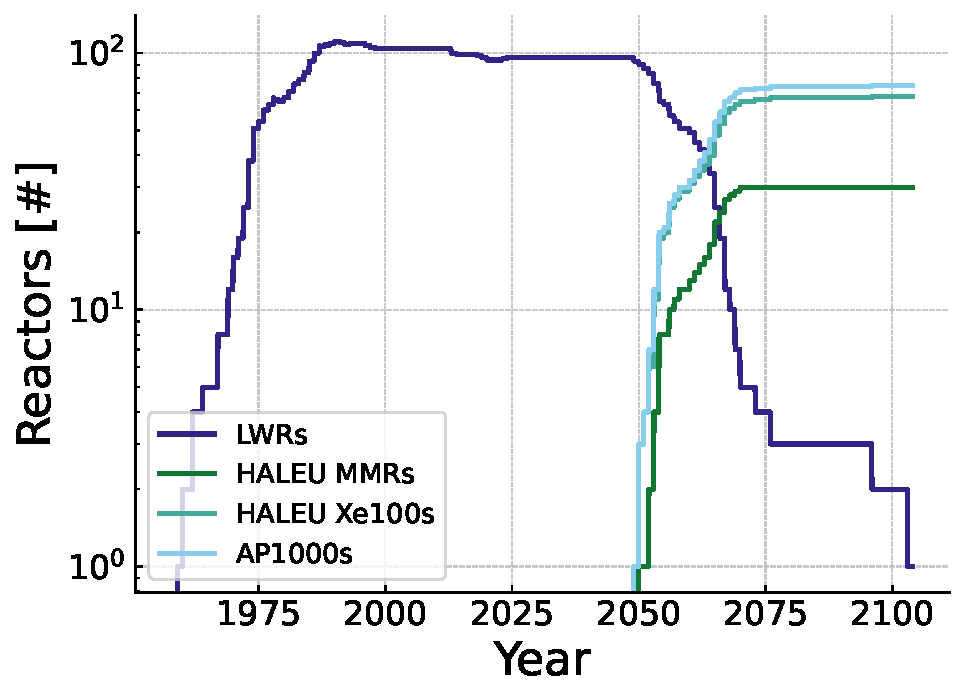
\includegraphics[width=0.495\textwidth]{images/results/reactors/multi_drng_reactors.pdf}
   }
    \hfill
    \subfloat[Double \label{fig:random_mf_d2_reactors}]{%
      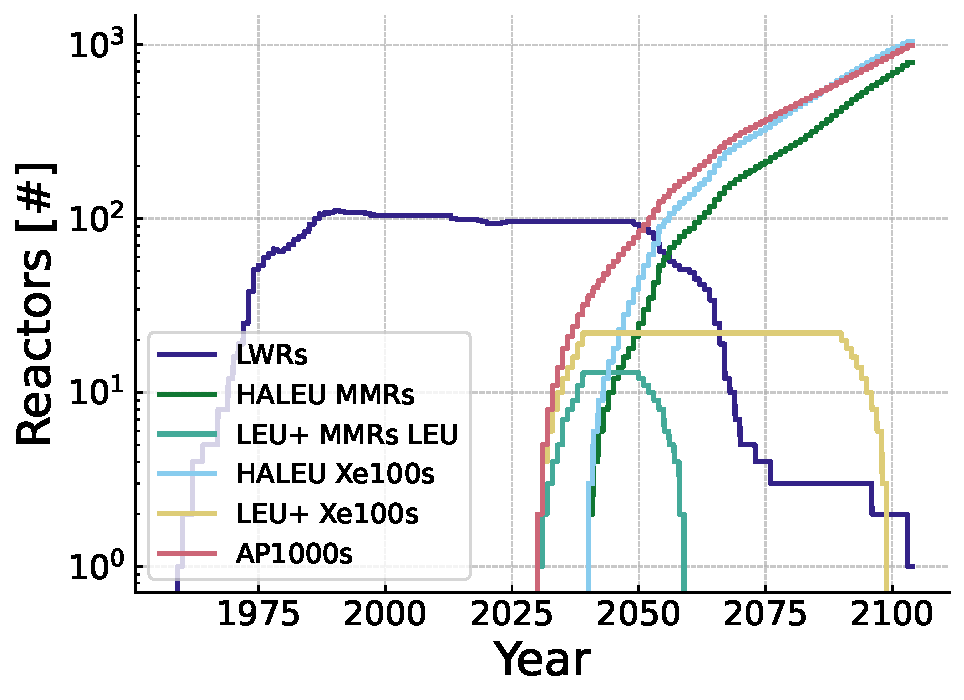
\includegraphics[width=0.495\textwidth]{images/results/reactors/multi_dr2_reactors.pdf}
   }
    \caption{Multi fuel random reactor deployment.}
    \label{fig:random_mf_reactors}
  \end{figure}

% talk about the rate of deployment

% talk about the context of expanding energy needs

% talk about the workers

\begin{figure}[H]
    \subfloat[No Growth \label{fig:random_of_ng_reactors}]{%
      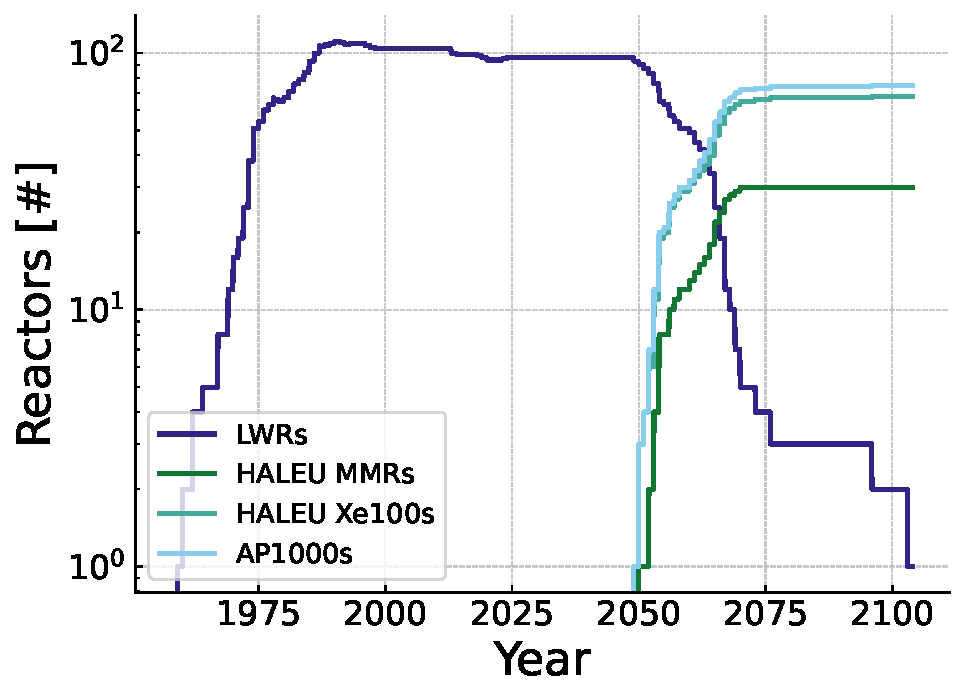
\includegraphics[width=0.495\textwidth]{images/results/reactors/one_drng_reactors.pdf}
   }
    \hfill
    \subfloat[Double \label{fig:random_of_d2_reactors}]{%
      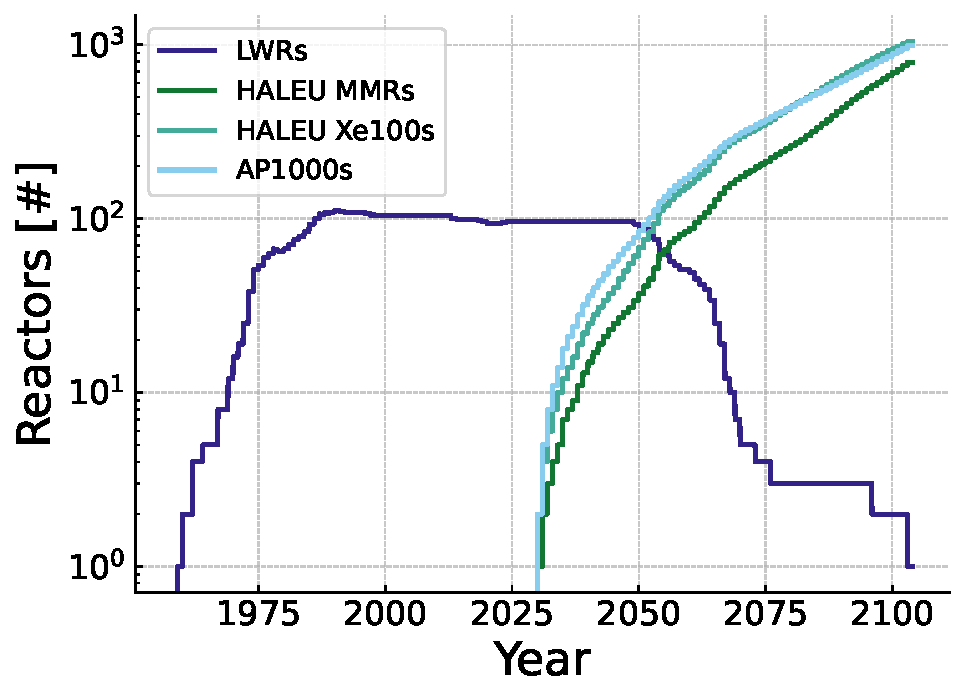
\includegraphics[width=0.495\textwidth]{images/results/reactors/one_dr2_reactors.pdf}
   }
    \caption{Single fuel random reactor deployment.}
    \label{fig:random_of_reactors}
  \end{figure}


In Table \ref{tab:random_reac_avg}, we show the average total number of reactors for the no growth and double scenarios in the single and multi fuel regimes. There is a 740\% increase in the number of AP1000s deployed going from the no growth scenario to the double scenario. The \gls{xe} reactors show a 249\% increase, while the \gls{mmr} reactors show a 62\% increase in the number of reactors deployed going from the no growth scenario to the double scenario in the single fuel regime. Unlike the reactor deployment under the greedy scheme in Section \ref{sec:greedy_reactors} and the initially random then greedy scheme in Section \ref{sec:rand_greed_reactors}, the random deployment scheme results for the single fuel and multi fuel regimes are not the same.

In the multi fuel regime, the AP1000 reactors show a 660\% increase in the number of reactors deployed going from the no growth scenario to the double scenario. The \gls{xe} reactors show a 746\% increase, while the \gls{mmr} reactors show a 1138\% increase in the number of reactors deployed going from the no growth scenario to the double scenario.

\begin{table}[H]
    \centering
    \caption{Average random total operating reactors by design.}
    \label{tab:random_reac_avg}
    \begin{tabular}{c c c c c}
       \hline
       Scenario & No Growth, Single & No Growth, Multi & Double, Single & Double, Multi  \\
       \hline
       \gls{haleu} fueled \glspl{mmr} & 131.613 & 17.267  & 213.707 & 210.24  \\
       \gls{leup} fueled \glspl{mmr}  & --      & --      & --      & 3.467   \\
       \gls{haleu} fueled \glspl{xe}  & 94.04   & 38.813  & 328.173 & 310.573 \\
       \gls{leup} fueled \glspl{xe}   & --      & --      & --      & 17.6    \\
       \gls{leu} fueled AP1000s       & 38.667  & 42.72   & 324.68  & 324.68  \\
       \hline
    \end{tabular}
\end{table}




\subsection{SWU Results}
\label{sec:random_swu}

% talk about the types of category facility

% talk about the SWU capacity

% show the total SWU capacity
\begin{figure}[H]
    \centering
    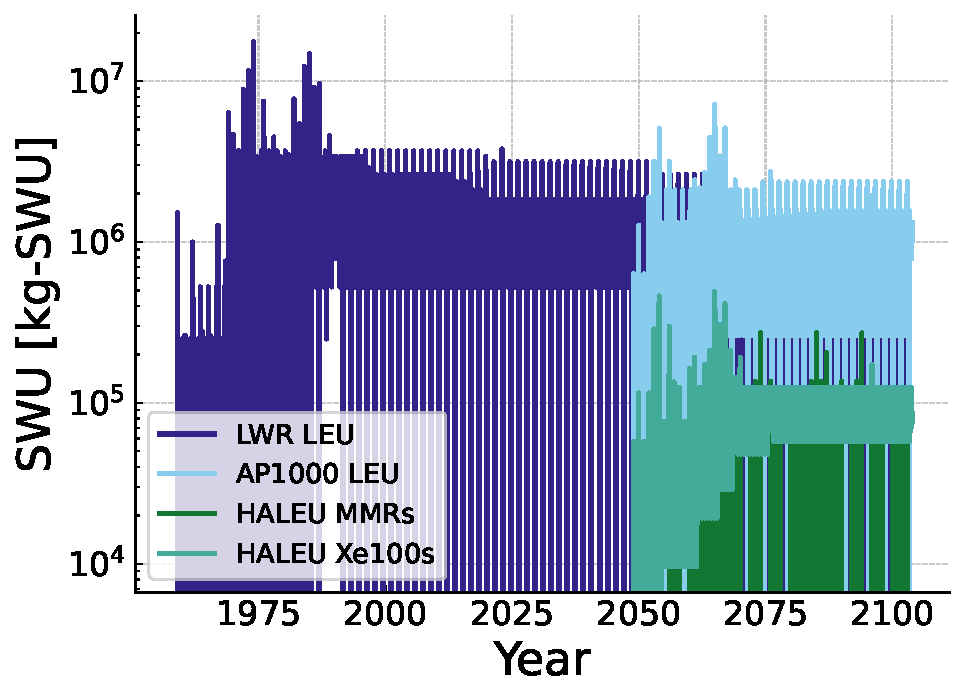
\includegraphics[scale=0.7]{images/results/swu/multi_drng_swu_by_fuel.pdf}
    \caption{Random reactor yearly SWU capacity.}
    \label{fig:swu_yearly_random}
\end{figure}

\begin{figure}[H]
  \subfloat[No Growth \label{fig:random_mf_ng_swu}]{%
    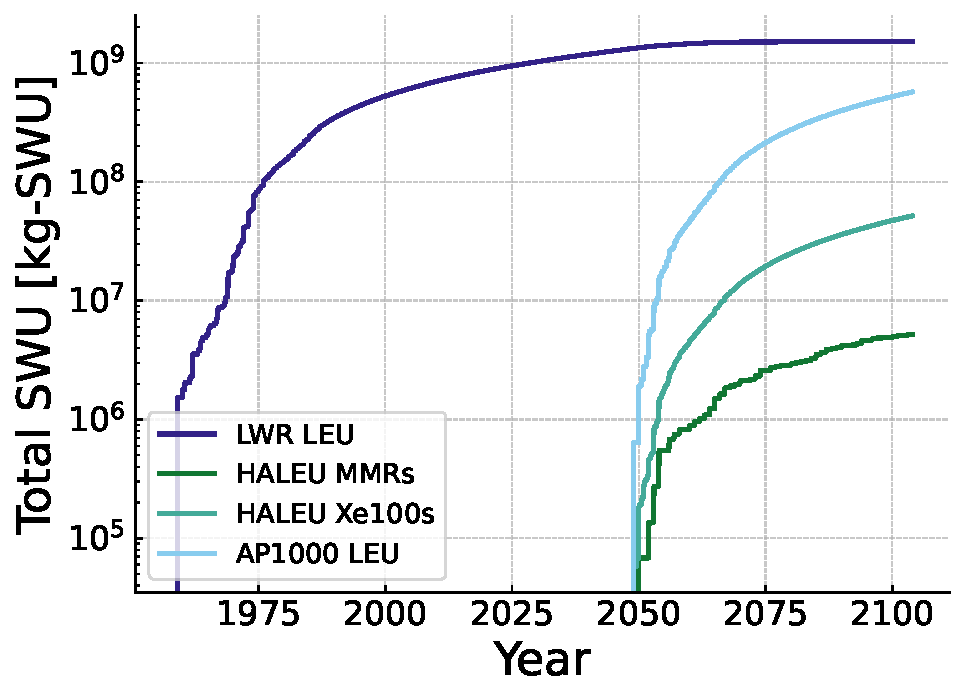
\includegraphics[width=0.495\textwidth]{images/results/swu/multi_drng_swu_cumulative_by_fuel.pdf}
 }
  \hfill
  \subfloat[Double \label{fig:random_mf_d2_swu}]{%
    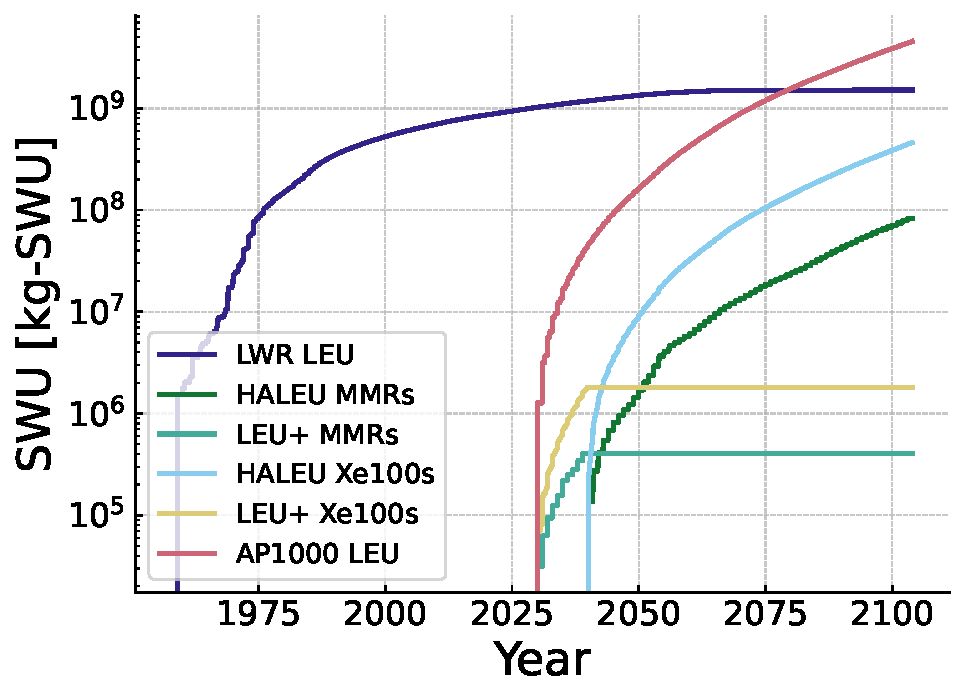
\includegraphics[width=0.495\textwidth]{images/results/swu/multi_dr2_swu_cumulative_by_fuel.pdf}
 }
  \caption{Random reactor multi fuel SWU.}
  \label{fig:random_mf_swu}
\end{figure}

% talk about international trade

\begin{figure}[H]
    \subfloat[No Growth \label{fig:random_of_ng_swu}]{%
      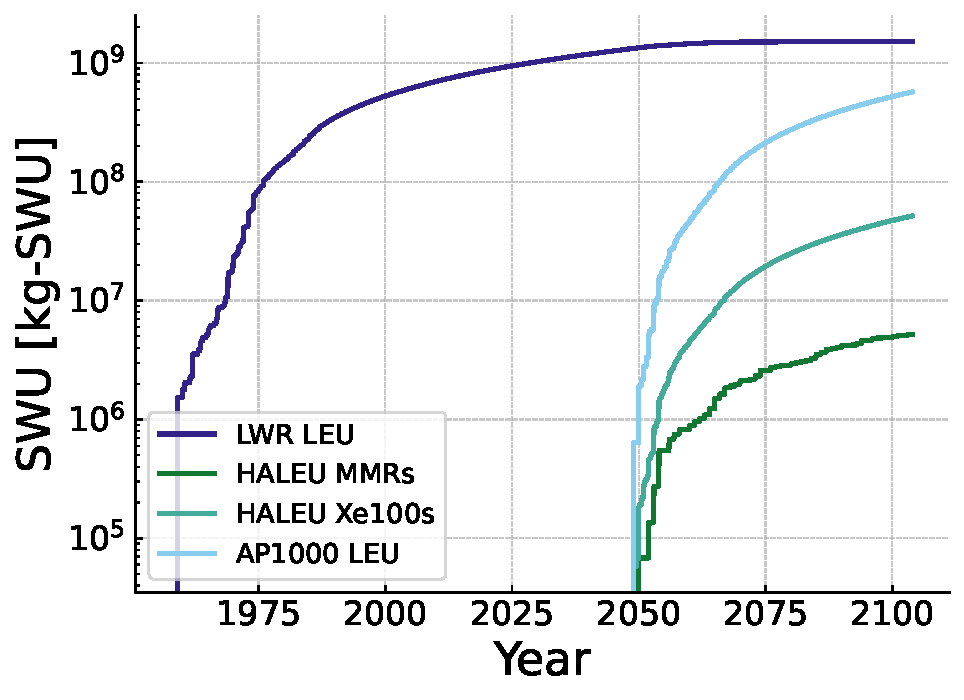
\includegraphics[width=0.495\textwidth]{images/results/swu/one_drng_swu_cumulative_by_fuel.pdf}
   }
    \hfill
    \subfloat[Double \label{fig:random_of_d2_swu}]{%
      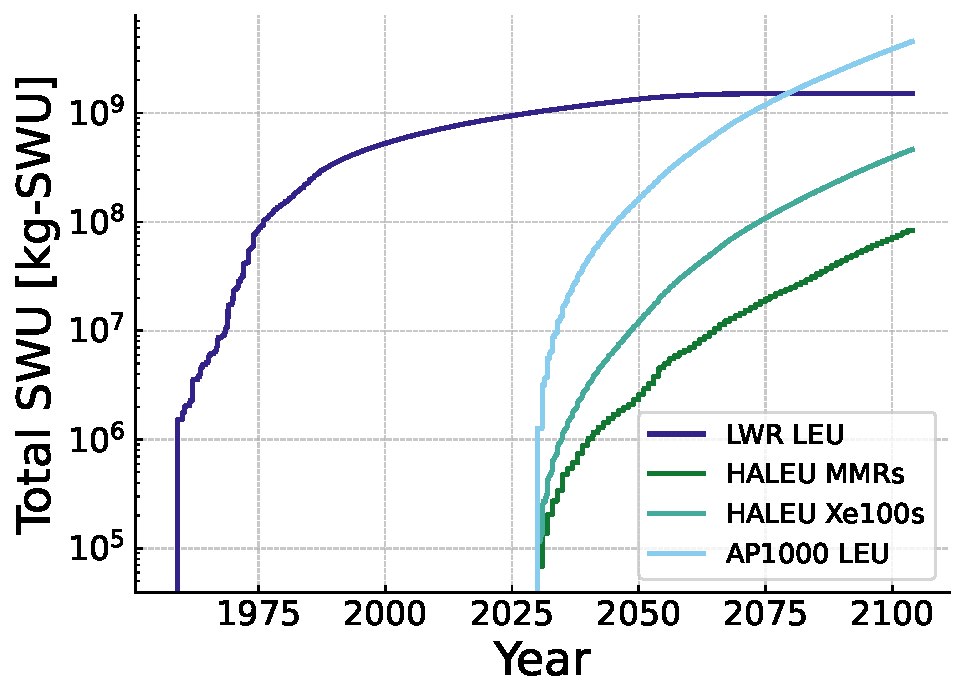
\includegraphics[width=0.495\textwidth]{images/results/swu/one_dr2_swu_cumulative_by_fuel.pdf}
   }
    \caption{Random reactor single fuel SWU.}
    \label{fig:random_of_swu}
\end{figure}


In Table \ref{tab:random_swu_avg}, we show the average total yearly \gls{swu} capacity for the no growth and double scenarios in the single and multi fuel regimes under the random deployment scheme. The \gls{xe} reactors show a 796\% increase in the average total yearly \gls{swu} capacity going from the no growth scenario to the double scenario in the single fuel regime. The \gls{mmr} reactors show a 1511\% increase in the average total yearly \gls{swu} capacity going from the no growth scenario to the double scenario in the single fuel regime. The AP1000 reactors show a 697\% increase in the average total yearly \gls{swu} capacity going from the no growth scenario to the double scenario in the single fuel regime.

\begin{table}[H]
    \centering
    \caption{Average random yearly SWU by design in k\gls{swu}.}
    \label{tab:random_swu_avg}
    \begin{tabular}{c c c c c}
       \hline
       Scenario & No Growth, Single & No Growth, Multi & Double, Single & Double, Multi  \\
       \hline
       \gls{mmr} \gls{haleu}   & 5.756   & 5.756   & 92.703    & 91.719   \\
       \gls{mmr} \gls{leup}    & --      & --      & --       & 0.453    \\
       \gls{xe} \gls{haleu}    & 57.327  & 57.327  & 513.746  & 510.388  \\
       \gls{xe} \gls{leup}     & --      & --      & --       & 2.021    \\
       AP1000 \gls{leu}        & 634.554 & 634.554 & 5050.323 & 5050.323 \\
       \hline
    \end{tabular}
\end{table}





\subsection{Fresh Fuel Results}
\label{sec:random_fresh}

% talk about the types of fuel

% show total fresh fuel

\begin{figure}[H]
    \subfloat[No Growth \label{fig:random_mf_ng_fresh}]{%
      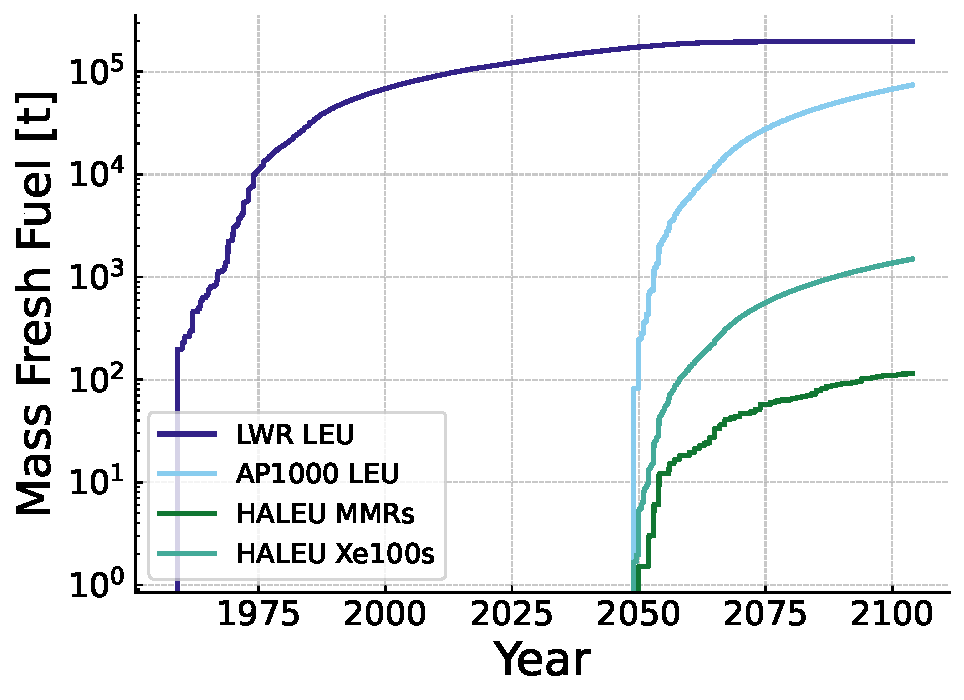
\includegraphics[width=0.495\textwidth]{images/results/fresh/multi_drng_fresh_fuel_cumulative_by_fuel.pdf}
   }
    \hfill
    \subfloat[Double \label{fig:random_mf_d2_fresh}]{%
      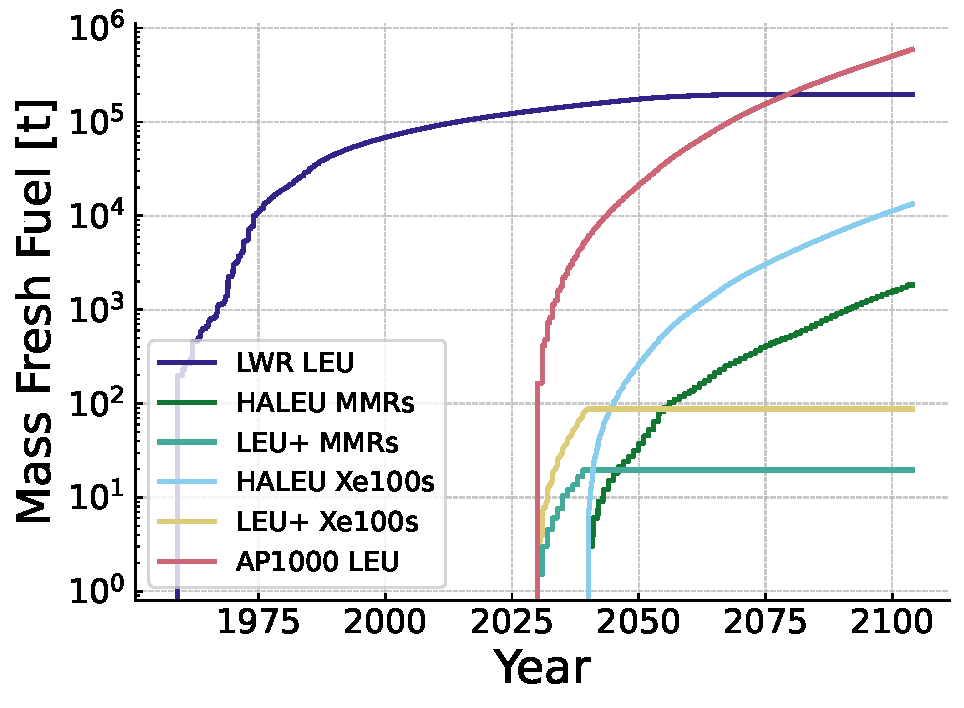
\includegraphics[width=0.495\textwidth]{images/results/fresh/multi_dr2_fresh_fuel_cumulative_by_fuel.pdf}
   }
    \caption{Random multi fresh fuel amount.}
    \label{fig:random_mf_fresh}
  \end{figure}

% talk about transportation of fuel


\begin{figure}[H]
    \subfloat[No Growth \label{fig:random_of_ng_fresh}]{%
      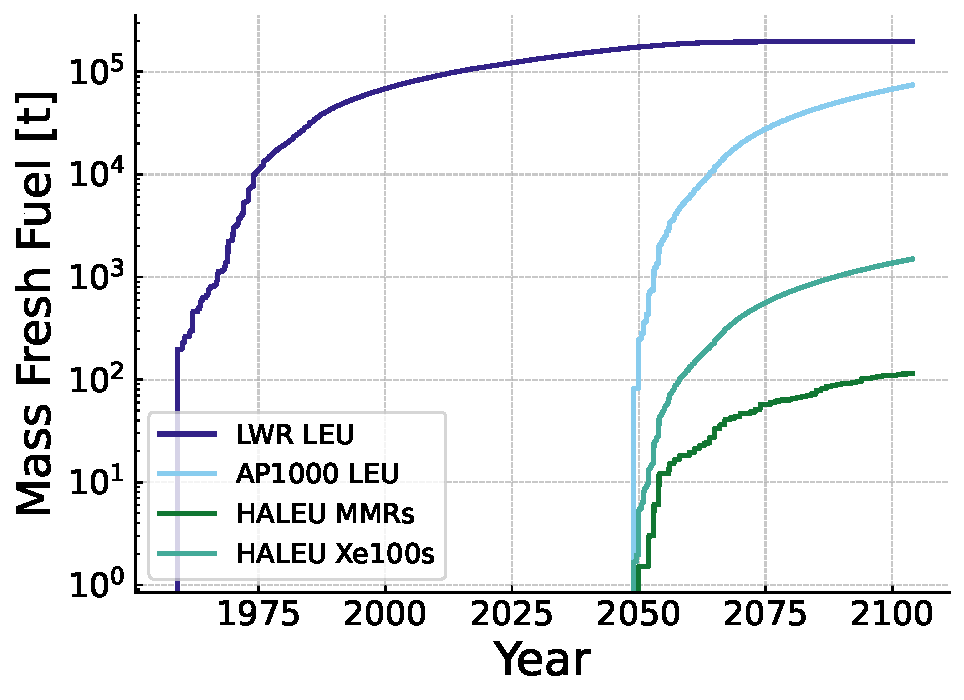
\includegraphics[width=0.495\textwidth]{images/results/fresh/one_drng_fresh_fuel_cumulative_by_fuel.pdf}
   }
    \hfill
    \subfloat[Double \label{fig:random_of_d2_fresh}]{%
      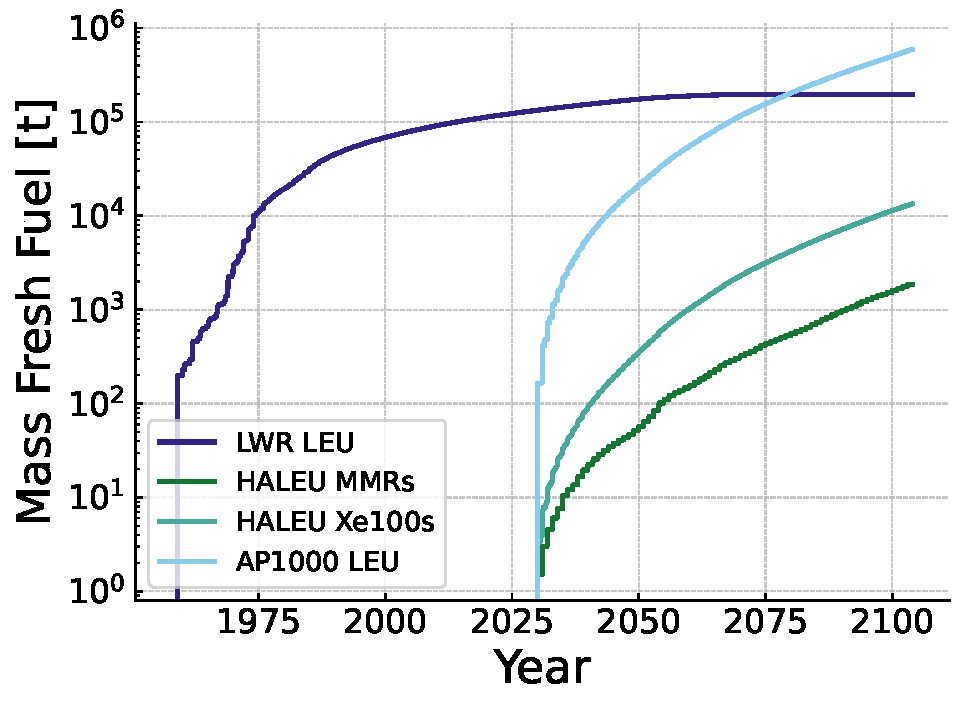
\includegraphics[width=0.495\textwidth]{images/results/fresh/one_dr2_fresh_fuel_cumulative_by_fuel.pdf}
   }
    \caption{Random single fresh fuel amount.}
    \label{fig:random_of_fresh}
\end{figure}




In Table \ref{tab:random_fresh_avg} we show the average total yearly fresh fuel for the no growth and double scenarios in the single and multi fuel regimes under the random deployment scheme. The \gls{xe} reactors show a 796\% increase in the average total yearly fresh fuel going from the no growth scenario to the double scenario in the single fuel regime. The \gls{mmr} reactors show a 1505\% increase in the average total yearly fresh fuel going from the no growth scenario to the double scenario in the single fuel regime. The AP1000 reactors show a 696\% increase in the average total yearly fresh fuel going from the no growth scenario to the double scenario in the single fuel regime.

\begin{table}[H]
    \centering
    \caption{Average random yearly fresh fuel by design in tonnes.}
    \label{tab:random_fresh_avg}
    \begin{tabular}{c c c c c}
       \hline
       Scenario & No Growth, Single & No Growth, Multi & Double, Single & Double, Multi  \\
       \hline
       \gls{mmr} \gls{haleu}   & 0.128    & 0.128   & 2.055    & 2.033    \\
       \gls{mmr} \gls{leup}    & --       & --      & --       & 0.107    \\
       \gls{xe} \gls{haleu}    & 1.663    & 1.663   & 14.904   & 14.806   \\
       \gls{xe} \gls{leup}     & --       & --      & --       & 0.022    \\
       AP1000 \gls{leu}        & 82.512   & 82.512  & 656.698  & 656.698  \\
       \hline
    \end{tabular}
\end{table}





\subsection{Used Fuel Results}
\label{sec:random_used}

% show total used fuel
\begin{figure}[H]
    \subfloat[No Growth \label{fig:random_mf_ng_used}]{%
      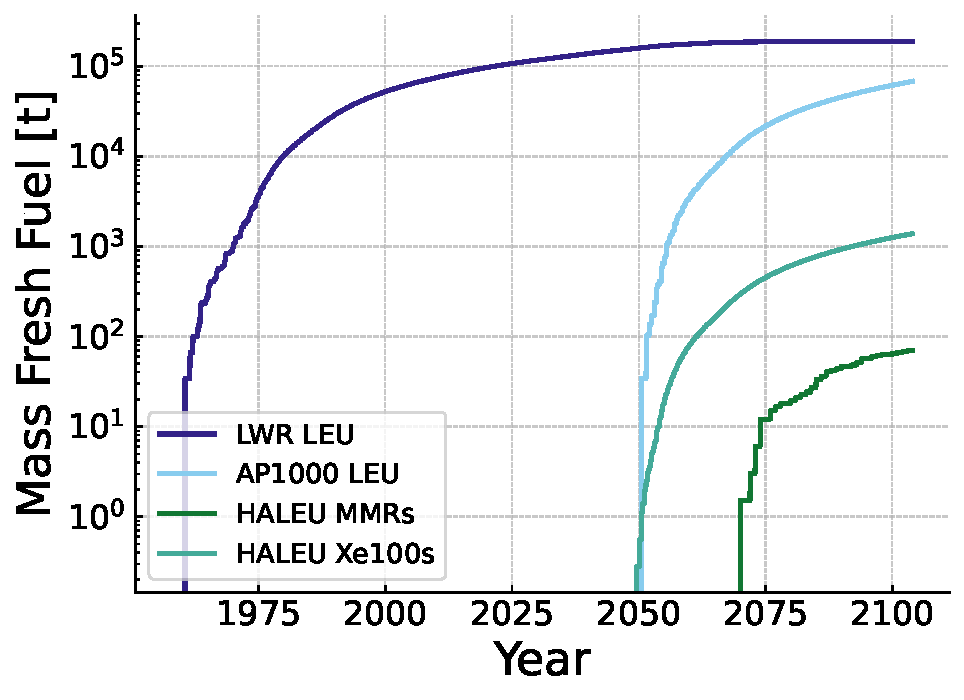
\includegraphics[width=0.495\textwidth]{images/results/used/multi_drng_used_fuel_cumulative_by_fuel.pdf}
   }
    \hfill
    \subfloat[Double \label{fig:random_mf_d2_used}]{%
      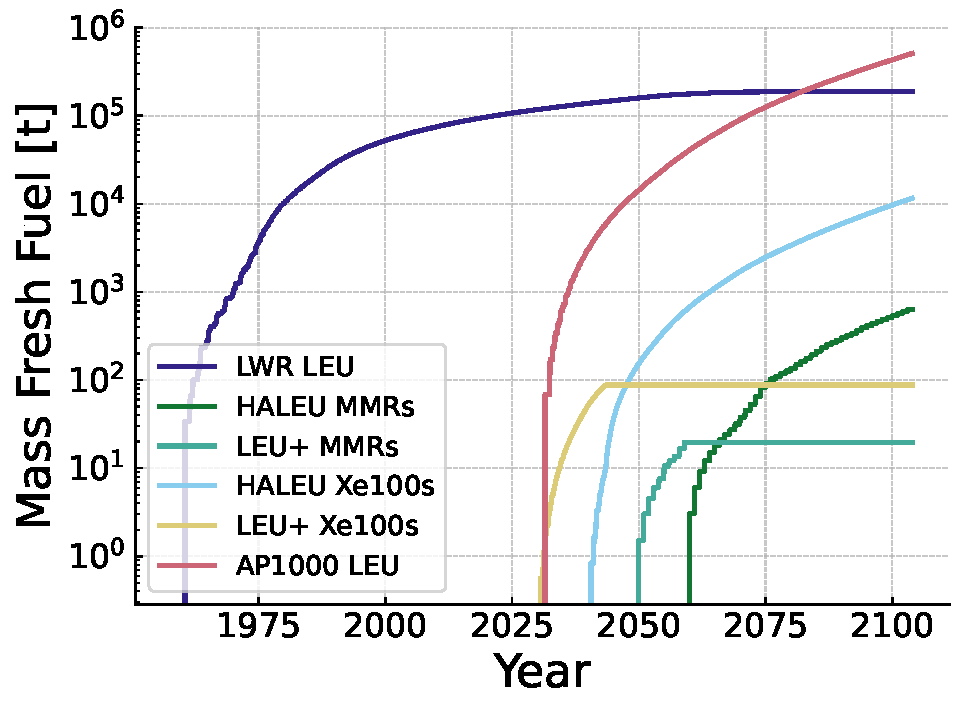
\includegraphics[width=0.495\textwidth]{images/results/used/multi_dr2_used_fuel_cumulative_by_fuel.pdf}
   }
    \caption{Random multi used fuel amount.}
    \label{fig:random_mf_used}
  \end{figure}


  \begin{figure}[H]
    \subfloat[No Growth \label{fig:random_of_ng_used}]{%
      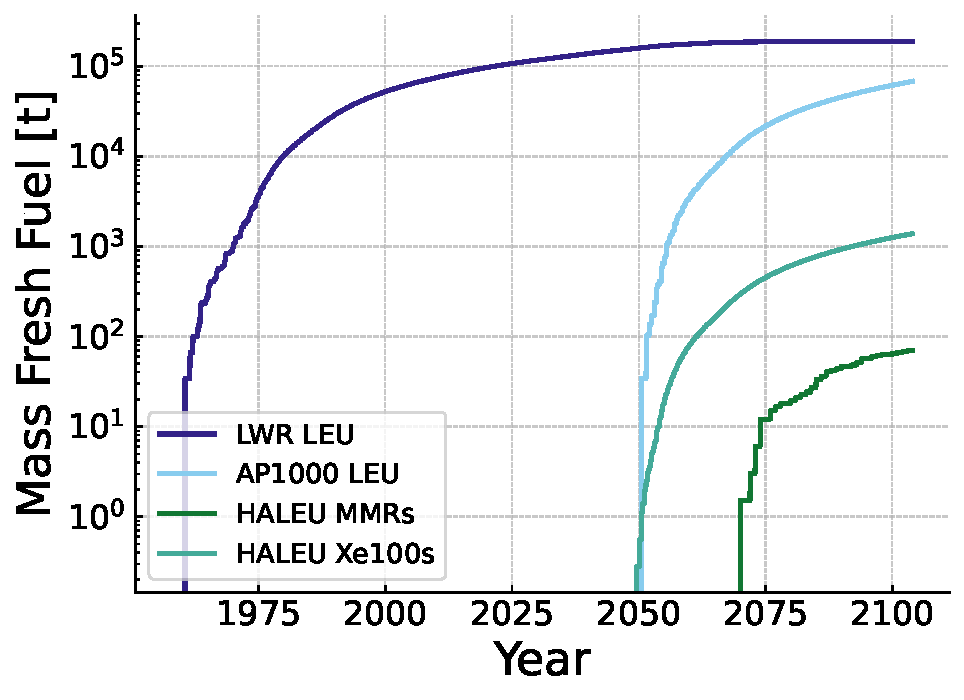
\includegraphics[width=0.495\textwidth]{images/results/used/one_drng_used_fuel_cumulative_by_fuel.pdf}
   }
    \hfill
    \subfloat[Double \label{fig:random_of_d2_used}]{%
      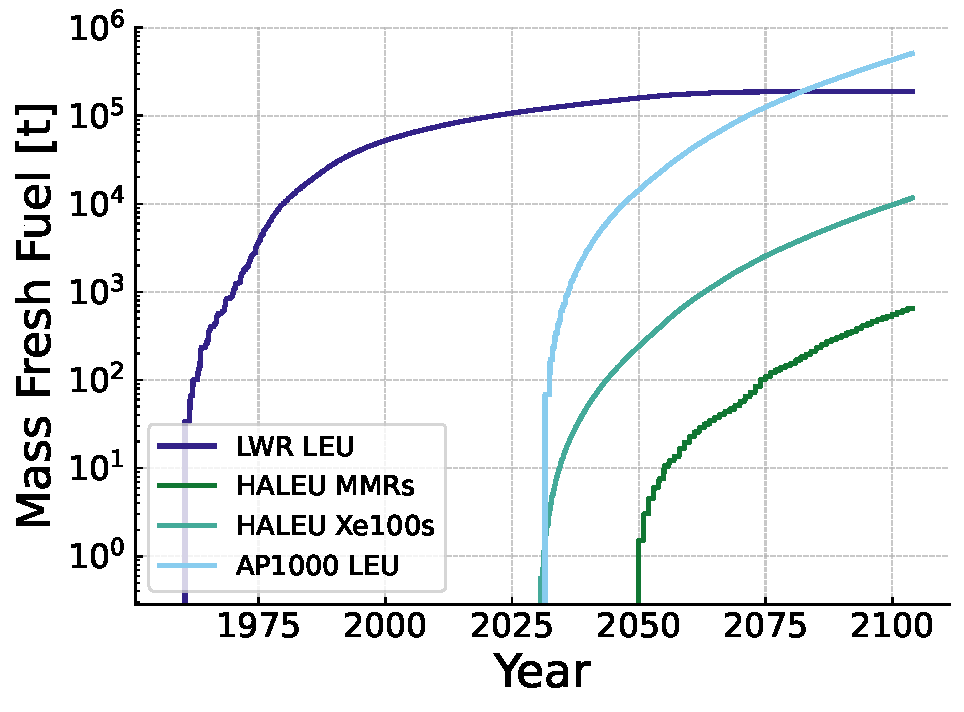
\includegraphics[width=0.495\textwidth]{images/results/used/one_dr2_used_fuel_cumulative_by_fuel.pdf}
   }
    \caption{Random single used fuel amount.}
    \label{fig:random_of_used}
\end{figure}


In Table \ref{tab:random_used_avg} we show the average total yearly used fuel for the no growth and double scenarios in the single and multi fuel regimes under the random deployment scheme. The \gls{xe} reactors show a 742\% increase in the average total yearly used fuel going from the no growth scenario to the double scenario in the single fuel regime. The \gls{mmr} reactors show a 838\% increase in the average total yearly used fuel going from the no growth scenario to the double scenario in the single fuel regime. The AP1000 reactors show a 649\% increase in the average total yearly used fuel going from the no growth scenario to the double scenario in the single fuel regime.

\begin{table}[H]
    \centering
    \caption{Average random yearly used fuel by design in tonnes.}
    \label{tab:random_used_avg}
    \begin{tabular}{c c c c c}
       \hline
       Scenario & No Growth, Single & No Growth, Multi & Double, Single & Double, Multi  \\
       \hline
       \gls{mmr} \gls{haleu}   & 0.077    & 0.077   & 0.722    & 0.700    \\
       \gls{mmr} \gls{leup}    & --       & --      & --       & 0.107    \\
       \gls{xe} \gls{haleu}    & 1.536    & 1.536   & 12.930   & 12.833   \\
       \gls{xe} \gls{leup}     & --       & --      & --       & 0.022    \\
       AP1000 \gls{leu}        & 75.638   & 75.638  & 566.239  & 566.239  \\
       \hline
    \end{tabular}
\end{table}

% talk about repositories